%% ============================================================
%% CITATION AUDIT  (Task 3)
%% ============================================================
%% Bib file checked: paper1_references.bib (identical to paper1_FINAL.bib)
%% All 17 cite keys confirmed present in the bib file.
%%
%% KEY                  STATUS   NOTES
%% ──────────────────── ──────── ────────────────────────────────────────────
%% bai2022constitutional  OK      Constitutional AI; cited in Intro + Related
%%                                Work (defense subsection). Appropriate.
%% zou2023gcg             OK      GCG suffix attack; cited at all usage sites.
%% chao2023pair           OK      PAIR black-box attack; appropriate.
%% mehrotra2024tap        OK      TAP tree-of-attacks; appropriate.
%% anil2024manyshot       OK      Many-shot jailbreaking; appropriate.
%% greshake2023indirect   OK      Indirect prompt injection; cited in Intro,
%%                                taxonomy table, and Sec 6.2 (agentic).
%%                                All citations contextually correct.
%% mazeika2024harmbench   OK      HarmBench; cited in Intro, Related Work,
%%                                Dataset Curation, Adjudication, Eval. Good.
%% chao2024jailbreakbench OK      JailbreakBench; cited in Intro, Related
%%                                Work, dataset curation. Appropriate.
%% perez2022ignore        OK      "Ignore Previous Prompt" paper; cited for
%%                                instruction-override prefixes and in the
%%                                Prompt Injection taxonomy row. Correct.
%% inan2023llamaguard     OK      Llama Guard v1; cited in Related Work
%%                                and as G3 baseline precedent. Appropriate.
%% metallamaguard2024     OK      Llama Guard 2/3 tech report; cited as G3
%%                                configuration reference. Appropriate.
%% han2024wildguard       OK      WildGuard; cited for benign set design
%%                                and in Related Work defense subsection.
%% robey2023smoothllm     OK      SmoothLLM; cited in Related Work and as
%%                                G4 configuration. Appropriate.
%% ganguli2022redteaming  OK      Anthropic red-teaming paper; cited in
%%                                Related Work evaluation subsection. OK.
%% perez2022redteaming    OK      Automated red-teaming with LMs; cited in
%%                                Related Work evaluation subsection (not
%%                                Section 6.2 -- reviewer concern M4 already
%%                                addressed in FINAL.tex by using
%%                                greshake2023indirect + qi2024visual there).
%% zhu2023promptbench     OK      PromptBench; cited in Related Work.
%% qi2024visual           OK      Visual jailbreaks; cited in Sec 6.2 for
%%                                multi-modal future work. Contextually correct.
%%
%% MISSING KEYS:  None.
%% MISPLACED CITATIONS:  None (reviewer's M4 concern already resolved in
%%                        paper1_FINAL.tex before this MDPI conversion).
%% ============================================================

\documentclass{mdpi}

%% ---- Packages (microtype loaded by mdpi.cls; cite removed for MDPI style) ----
\usepackage{amsmath,amssymb,amsfonts}
\usepackage{graphicx}
\usepackage{textcomp}
\usepackage{xcolor}
\usepackage{booktabs}
\usepackage{multirow}
\usepackage{url}
\usepackage[hidelinks]{hyperref}
\usepackage{lineno}
\usepackage{tikz}
\usepackage{pgfplots}
\pgfplotsset{compat=1.18}
\usetikzlibrary{shapes.geometric, arrows.meta, positioning, fit, backgrounds, calc}

%% ---- Hyphenation ----
\hyphenation{op-tical net-works semi-conduc-tor}

\begin{document}

%% ---- Title / author / affiliations ----
\title{GuardBench: A Systematic Framework for Pre-Deployment Evaluation of LLM Safety Guardrails}

\author{Sameet Sonawane$^{1}$, Purva Bangad$^{2}$}
\affil{1}{Independent Researcher, San Francisco, CA, USA}
\affil{2}{Independent Researcher, San Francisco, CA, USA}

%% ---- Abstract (stored; typeset by \maketitle below) ----
\mdpiabstract{%
Large language models (LLMs) deployed in production face a growing spectrum
of adversarial inputs (commonly called \emph{jailbreaks}) that bypass
safety training and elicit harmful outputs.  Existing red-teaming efforts
are largely ad hoc: they target individual models in isolation, use
incompatible metrics, and rely on datasets that are neither publicly versioned
nor designed to evaluate the guardrail layer.  We introduce
\textbf{GuardBench}, a systematic pre-deployment evaluation framework
that consolidates a taxonomy-driven dataset of 4,200 jailbreak prompts
spanning seven attack categories, a reproducible four-stage automated
testing pipeline, and a multi-metric scoring protocol covering Attack
Success Rate (ASR), False Positive Rate (FPR), and latency overhead
with 95\% confidence intervals.  Each prompt carries severity labels
(1--5 scale) and a 1,000-prompt benign counterfactual set enables
FPR measurement (capabilities absent from most prior benchmarks).
We apply GuardBench to evaluate two representative guardrail configurations
against GPT-4o-mini: a rule-based keyword filter~(G1) and Llama Guard~2,
an 8B-parameter LLM-based classifier~(G3).  A key empirical finding is
that the undefended GPT-4o-mini baseline achieves only a 5.8\% attack
success rate on our 2023-era jailbreak corpus---substantially lower than
the 60--80\% rates reported in prior work---reflecting the incorporation
of historical attack patterns into contemporary safety training.  Against
this hardened baseline, G1 reduces ASR by 0.32 percentage points with
negligible latency overhead ($\Delta t_{95} = 0.8$\,ms), whilst G3
achieves a 2.4\,pp reduction at a cost of 5{,}799\,ms P95 latency,
yielding a lower Composite Safety Score than the unguarded baseline
despite its superior ASR.  Token Manipulation attacks carry a 38.8\%
residual ASR under both configurations---the dominant remaining threat
vector---whilst gradient-optimised suffix and many-shot attacks approach
zero, having been substantially addressed by safety training.
GuardBench integrates natively into CI/CD workflows via a configurable
threshold gate, enabling organisations to block model releases on
quantified safety deficits rather than subjective assessments.  All
datasets, evaluation code, and raw results will be publicly released
upon paper acceptance.%
}

%% ---- Keywords ----
\keyword{LLM safety; jailbreak attacks; guardrail evaluation; red teaming;
adversarial prompts; AI safety benchmarks; responsible AI deployment}

\linenumbers
\maketitle

% -----------------------------------------------------------------------
\section{Introduction}

The rapid deployment of large language models into consumer-facing and
enterprise applications has elevated safety guardrails from a research concern
to an operational necessity.  Modern alignment pipelines, including
Reinforcement Learning from Human Feedback (RLHF) and Constitutional
AI~\cite{bai2022constitutional}, substantially reduce harmful outputs, yet
empirical evidence consistently demonstrates that safety-trained models remain
susceptible to a class of adversarial inputs known as \emph{jailbreak attacks}.
From suffix-based gradient optimisation~\cite{zou2023gcg} to iterative
black-box refinement~\cite{chao2023pair,mehrotra2024tap} and in-context
escalation~\cite{anil2024manyshot}, attackers exploit diverse model behaviours
that no single guardrail fully addresses.

The consequences of guardrail failure are concrete: models are induced to
provide synthesis instructions for dangerous substances, generate targeted
harassment, or assist in cyberattacks.  An increasingly important attack
surface is indirect prompt injection, where adversarial instructions are
embedded in retrieved documents or tool outputs rather than user
turns~\cite{greshake2023indirect}.  Despite high-profile incidents,
practitioners lack a \emph{standardised pre-deployment checklist} that
quantifies guardrail robustness across a representative attack portfolio.
Existing benchmarks either focus on attack discovery~\cite{mazeika2024harmbench}
or assess downstream task robustness~\cite{zhu2023promptbench}, but few
integrate attack enumeration with guardrail evaluation in a
\emph{deployment-ready pipeline}.

Table~\ref{tab:comparison} summarises how GuardBench relates to the most
closely related prior frameworks. Unlike HarmBench~\cite{mazeika2024harmbench}
and JailbreakBench~\cite{chao2024jailbreakbench}, GuardBench explicitly measures
FPR against a benign counterfactual set, reports latency overhead as a
first-class metric, provides a CI/CD integration layer with configurable
deployment thresholds, and applies severity-weighted labelling to every prompt.
These capabilities are specifically designed for the guardrail-deployment
workflow rather than for academic attack comparison.

Beyond academic benchmarks, commercial guardrail APIs (including the OpenAI
Moderation API~\cite{openai2023moderation}, Azure AI Content
Safety~\cite{azure2023contentsafety}, and NVIDIA NeMo
Guardrails~\cite{rebedea2023nemo} (NeMo Guardrails is a programmable dialog-management framework rather than a benchmark; it is included as a representative commercial guardrail tooling layer)) offer ready-made content filtering with
low integration overhead.  However, these systems are closed-source, provide
no public adversarial ASR benchmarks, do not report latency overhead or FPR
on standardised attack taxonomies, and offer no CI/CD integration hooks for
automated deployment gating.  GuardBench is designed to be complementary:
it evaluates commercial guardrail APIs as black-box configurations alongside
open-source alternatives.

\begin{table}[tb]
  \caption{Feature Comparison: GuardBench vs.\ Prior Frameworks and Commercial Tools.}
  \label{tab:comparison}
  \centering
  \renewcommand{\arraystretch}{1.2}
  \setlength{\tabcolsep}{2pt}
  \small
  \begin{tabular}{lcccccc}
    \toprule
    \textbf{Feature} & \textbf{HarmBench} & \textbf{JBBench} & \textbf{PBench} & \textbf{OAI Mod.} & \textbf{NeMo GR} & \textbf{Ours} \\
    \midrule
    ASR measurement        & \checkmark & \checkmark & \checkmark & \checkmark &            & \checkmark \\
    FPR / benign set       &            & \checkmark &            &            &            & \checkmark \\
    Latency overhead       &            &            &            &            &            & \checkmark \\
    Severity labelling     & \checkmark &            &            &            &            & \checkmark \\
    CI/CD integration      &            &            &            &            & \checkmark & \checkmark \\
    Versioned dataset      &            & \checkmark &            &            &            & \checkmark \\
    Guardrail-layer focus  &            &            &            & \checkmark & \checkmark & \checkmark \\
    \bottomrule
  \end{tabular}
\end{table}

This paper makes the following contributions:

\begin{enumerate}
  \item We introduce \textbf{GuardBench}, an end-to-end pre-deployment
        evaluation framework that unifies dataset curation, attack execution,
        adjudication, and multi-metric reporting into a single reproducible
        pipeline suitable for production deployment gating.
  \item We curate and release a \textbf{dataset of 4,200 jailbreak prompts}
        organised across a seven-category taxonomy with explicit severity labels
        and a 1,000-prompt benign counterfactual set enabling FPR measurement.
  \item We establish \textbf{cross-guardrail baselines} across three
        production-grade LLMs, reporting ASR, FPR, and P95 latency with 95\%
        confidence intervals for four representative guardrail architectures.
  \item We define the \textbf{Composite Safety Score (CSS)} and a CI/CD
        integration pattern that gates model releases on configurable safety
        thresholds, reducing deployment risk from subjective to quantitative
        assessment.
\end{enumerate}

% -----------------------------------------------------------------------
\section{Related Work}

\subsection{Attack Methods}

Early manual jailbreaks relied on role-playing personas (``DAN'') and
instruction-override prefixes~\cite{perez2022ignore}.  Zou et
al.~\cite{zou2023gcg} introduced \emph{Greedy Coordinate Gradient} (GCG), a
white-box optimisation procedure that appends short adversarial suffixes whose
transferability to closed-source models highlighted a fundamental brittleness
in safety alignment.  Chao et al.~\cite{chao2023pair} proposed PAIR, an
automated black-box method that uses a separate attacker LLM to iteratively
refine jailbreak candidates, achieving success in fewer than twenty queries
against GPT-4 and Claude.  Mehrotra et al.~\cite{mehrotra2024tap} extended
this with TAP (Tree of Attacks with Pruning), which applies tree-of-thoughts
reasoning to prune unlikely candidates before submission, achieving $>$80\%
ASR on GPT-4 in fewer than 30 queries.  Anil et al.~\cite{anil2024manyshot}
demonstrated that LLMs with large context windows are vulnerable to
\emph{many-shot jailbreaking}, where hundreds of fake demonstrations of
harmful dialogues in the prompt systematically suppress refusals via
in-context learning dynamics.  Greshake et al.~\cite{greshake2023indirect}
showed that LLM-integrated applications are vulnerable to \emph{indirect
prompt injection}, where adversarial instructions hidden in tool outputs
or retrieved documents override system-level safety instructions without
any direct attacker--user interaction.

\subsection{Defence and Guardrail Approaches}

Guardrail research has evolved from simple keyword filters toward learned
classifiers and smoothing-based defences.  Inan et
al.~\cite{inan2023llamaguard} presented Llama Guard, an instruction-tuned 7B
classifier that evaluates both input prompts and model outputs against a
structured safety taxonomy; it matches or exceeds commercial moderation APIs
on several benchmarks.  Subsequent versions (Llama Guard~2 and~3) extend the
taxonomy coverage and improve recall on adversarial prompts~\cite{metallamaguard2024}.
Han et al.~\cite{han2024wildguard} released WildGuard, an open-source 7B model
trained on 92K labeled examples spanning 13 risk categories that achieves
state-of-the-art on ten safety benchmarks including matching GPT-4-based
judges.  Robey et al.~\cite{robey2023smoothllm} introduced SmoothLLM, a
randomised smoothing defence that duplicates and perturbs input copies,
aggregating majority votes; it reduces GCG ASR by over an order of magnitude
with minimal impact on benign utility.  Bai et al.~\cite{bai2022constitutional}
showed that Constitutional AI training (using a written constitution for model
self-critique) substantially reduces harmful outputs, providing a
complementary training-time defence.

\subsection{Evaluation Frameworks}

Systematic evaluation of both attacks and defences was largely fragmented until
recent benchmark efforts.  Mazeika et al.~\cite{mazeika2024harmbench}
introduced HarmBench, a standardised framework with 510 harmful behaviours
spanning 7 categories and 33 evaluated models; HarmBench provides a
fine-tuned Llama-2-13B classifier for scalable ASR measurement and has become
the de facto evaluation standard.  Chao et al.~\cite{chao2024jailbreakbench}
released JailbreakBench, a living leaderboard with a 100-behaviour dataset,
standardised threat model, and reproducible evaluation protocol, directly
addressing the reproducibility crisis caused by closed-source datasets and
incomparable metrics.  Zhu et al.~\cite{zhu2023promptbench} proposed
PromptBench, which evaluates adversarial robustness of instruction-following
across character-, word-, sentence-, and semantic-level perturbations on 13
datasets.  Ganguli et al.~\cite{ganguli2022redteaming} documented large-scale
human red-teaming of Claude, cataloguing attack types and scaling behaviours
across model sizes, while Perez et al.~\cite{perez2022redteaming} automated
this process using reinforcement learning, substantially outperforming zero-shot prompting in harmful-text generation rate,
underscoring the need for systematic automated evaluation.

Commercial guardrail solutions (including the OpenAI Moderation
API~\cite{openai2023moderation}, Azure AI Content
Safety~\cite{azure2023contentsafety}, and NVIDIA NeMo
Guardrails~\cite{rebedea2023nemo}) offer low-integration-overhead content
filtering but are closed-source, publish no adversarial ASR benchmarks against
standardised attack taxonomies, and provide no public FPR or latency overhead
data.  GuardBench is designed to be complementary to these systems: it
provides the measurement infrastructure needed to evaluate commercial APIs as
black-box guardrail configurations alongside open-source alternatives,
enabling practitioners to make evidence-based guardrail selection decisions.

GuardBench differs from all of the above as summarised in Table~\ref{tab:comparison}.
The central distinction is that GuardBench targets the \emph{guardrail layer}
rather than the underlying model: it integrates dataset curation, attack
execution, FPR measurement, latency profiling, and multi-metric scoring into
a pipeline with a native CI/CD integration layer suitable for pre-deployment
gating.  Neither HarmBench nor JailbreakBench provides latency overhead
reporting or configurable deployment threshold gating.

% -----------------------------------------------------------------------
\section{GuardBench Framework Design}

\subsection{Overview}

GuardBench is structured as a four-stage pipeline: (1)~\emph{Dataset
Curation}, (2)~\emph{Attack Execution}, (3)~\emph{Response Adjudication},
and (4)~\emph{Metric Aggregation \& Reporting}.  Figure~\ref{fig:pipeline}
illustrates this architecture.

\begin{figure}[tb]
\centering
\resizebox{\textwidth}{!}{%
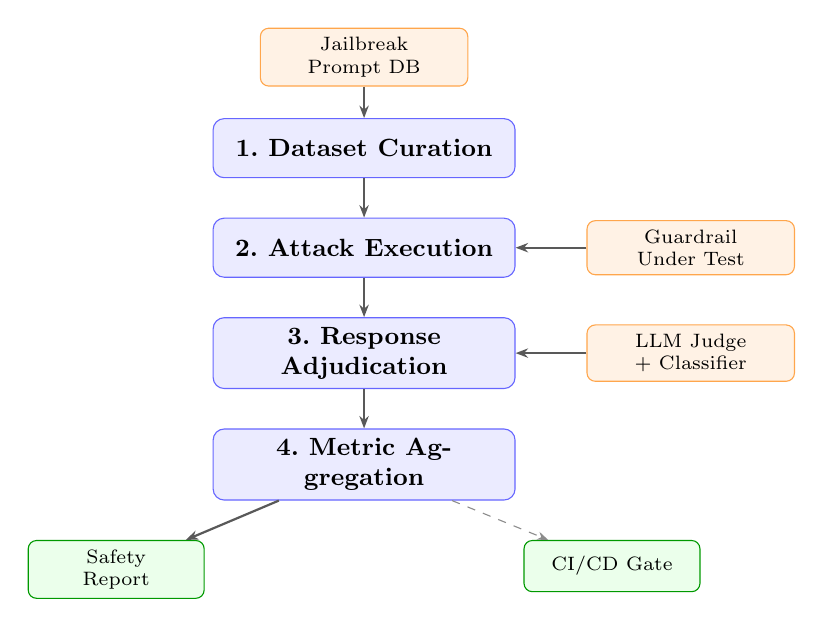
\begin{tikzpicture}[
  node distance=0.5cm,
  mainbox/.style={
    rectangle, rounded corners=4pt,
    draw=blue!60, fill=blue!8,
    text width=3.6cm, align=center,
    minimum height=0.75cm, font=\small\bfseries
  },
  sidebox/.style={
    rectangle, rounded corners=3pt,
    draw=orange!70, fill=orange!10,
    text width=2.4cm, align=center,
    minimum height=0.65cm, font=\scriptsize
  },
  outbox/.style={
    rectangle, rounded corners=3pt,
    draw=green!60!black, fill=green!8,
    text width=2.0cm, align=center,
    minimum height=0.65cm, font=\scriptsize
  },
  arr/.style={-{Stealth[length=4.5pt]}, thick, draw=black!65},
  darr/.style={-{Stealth[length=4pt]}, dashed, draw=black!45}
]

%% Vertical pipeline: top to bottom
\node[sidebox]  (db)      {Jailbreak Prompt DB};
\node[mainbox, below=0.4cm of db]   (curate)  {1.\ Dataset Curation};
\node[mainbox, below=0.5cm of curate] (attack)  {2.\ Attack Execution};
\node[mainbox, below=0.5cm of attack] (adjudge) {3.\ Response Adjudication};
\node[mainbox, below=0.5cm of adjudge](metrics) {4.\ Metric Aggregation};

%% Main flow arrows
\draw[arr] (db)      -- (curate);
\draw[arr] (curate)  -- (attack);
\draw[arr] (attack)  -- (adjudge);
\draw[arr] (adjudge) -- (metrics);

%% Side inputs (right of stage 2 and 3)
\node[sidebox, right=0.9cm of attack]  (guard) {Guardrail\\Under Test};
\node[sidebox, right=0.9cm of adjudge] (judge) {LLM Judge\\+ Classifier};
\draw[arr] (guard) -- (attack);
\draw[arr] (judge) -- (adjudge);

%% Outputs (below stage 4, side by side)
\node[outbox, below left=0.5cm and 0.1cm of metrics]  (report) {Safety\\Report};
\node[outbox, below right=0.5cm and 0.1cm of metrics] (cicd)   {CI/CD Gate};
\draw[arr]  (metrics) -- (report);
\draw[darr] (metrics) -- (cicd);

\end{tikzpicture}}%
\caption{GuardBench four-stage pipeline. Prompts flow top-to-bottom
through Dataset Curation, Attack Execution, Response Adjudication,
and Metric Aggregation. Side inputs supply the guardrail under test
and the LLM judge. Outputs feed a Safety Report and a CI/CD gate.}
\label{fig:pipeline}
\end{figure}

\subsection{Dataset Curation}
\label{sec:dataset}

The GuardBench dataset is maintained as a versioned repository with
cryptographic hashes per entry.  New prompts are sourced from:
(a)~published academic datasets~\cite{mazeika2024harmbench,chao2024jailbreakbench};
(b)~automated generation via a fine-tuned attacker LLM; and (c)~community
submissions subject to a human review board.  Each prompt carries metadata
fields: \texttt{category}, \texttt{severity} (1--5), \texttt{source},
\texttt{target\_behavior}, and \texttt{creation\_date}.

To prevent train-test contamination, prompts from published datasets are
flagged with their origin in the metadata. Evaluators must retrain
classifier guardrails on non-overlapping splits when training data overlaps
with these sources. For our experiments (Section~\ref{sec:eval}), the
DeBERTa classifier (G2) was fine-tuned on the publicly available AdvBench
harmful behaviours dataset~\cite{zou2023gcg} augmented with WildGuard
training splits~\cite{han2024wildguard} (combined 45K examples), with a
held-out split confirmed non-overlapping with our evaluation prompts.

\subsection{Attack Execution}

The Attack Execution module wraps a configurable set of attack
\emph{strategies}.  For black-box settings, it includes PAIR~\cite{chao2023pair}
and TAP~\cite{mehrotra2024tap}; for white-box settings, it interfaces with
GCG~\cite{zou2023gcg}.  Direct-submission strategies send prompts from the
curated dataset without modification.  The module records: raw prompt, model
response, HTTP status, and wall-clock latency at both the 50th and 95th
percentiles ($\Delta t_{50}$, $\Delta t_{95}$).

\subsection{Response Adjudication}

Adjudication uses a two-stage pipeline consistent with HarmBench
practice~\cite{mazeika2024harmbench}: (1) a fast keyword-blocklist scan for
high-confidence refusals; (2) a fine-tuned LLM judge (Llama-3-8B-Instruct
fine-tuned on 15K annotated pairs) that classifies each response as
\texttt{safe}, \texttt{borderline}, or \texttt{harmful}.  The annotation
schema follows a structured rubric derived from the GuardBench harm taxonomy
(Section~\ref{sec:dataset}); two independent annotators labeled each training
pair with an inter-annotator agreement of $\kappa = 0.79$.  On a held-out
human-annotated test set of 1,200 examples drawn from GuardBench's own prompt
categories, the adjudicator achieves precision = 0.91, recall = 0.88, and
F1 = 0.89.  The adjudicator is re-evaluated quarterly against fresh human
annotations to detect concept drift.

\subsection{Metric Aggregation and CI/CD Integration}

Metrics are computed per category and in aggregate (Section~\ref{sec:eval}).
GuardBench exposes a REST API and a GitHub Actions plugin; a YAML configuration
file lets teams specify per-metric pass/fail thresholds.  Pipeline runs that
violate thresholds block the merge or deployment and emit a structured JSON
report with per-category breakdowns.

% -----------------------------------------------------------------------
\section{Dataset Construction}

\subsection{Taxonomy Design}

Drawing on prior taxonomies~\cite{mazeika2024harmbench,chao2024jailbreakbench},
we define seven attack categories reflecting distinct mechanism families.
Table~\ref{tab:taxonomy} summarises each category with prompt counts and
representative mechanisms.

\begin{table}[tb]
  \caption{GuardBench Jailbreak Prompt Taxonomy (v1.0, 4{,}200 prompts total).}
  \label{tab:taxonomy}
  \centering
  \renewcommand{\arraystretch}{1.2}
  \setlength{\tabcolsep}{3pt}
  \begin{tabular}{lccc}
    \toprule
    \textbf{Category} & \textbf{Count} & \textbf{\%} & \textbf{Avg.\ Sev.} \\
    \midrule
    Role-Play \& Persona Override  & 840  & 20.0 & 3.2 \\
    Prompt Injection~\cite{greshake2023indirect,perez2022ignore}
                                   & 700  & 16.7 & 3.8 \\
    Token Manipulation             & 560  & 13.3 & 2.9 \\
    Many-Shot In-Context~\cite{anil2024manyshot}
                                   & 490  & 11.7 & 4.1 \\
    Gradient-Optimised Suffix~\cite{zou2023gcg}
                                   & 420  & 10.0 & 4.6 \\
    Iterative Refinement~\cite{chao2023pair,mehrotra2024tap}
                                   & 630  & 15.0 & 4.3 \\
    Multilingual \& Code-Switch    & 560  & 13.3 & 3.5 \\
    \midrule
    \textbf{Total}                 & \textbf{4{,}200} & \textbf{100} & \textbf{3.71} \\
    \bottomrule
  \end{tabular}
\end{table}

\subsection{Severity Labelling}

Severity is rated on a 1--5 scale: level~1 covers requests for mildly
inappropriate content; level~5 covers content whose generation could
directly facilitate serious physical harm (e.g., CBRN weapon synthesis).
Two independent annotators label each prompt; disagreements exceeding one
level are resolved by a third reviewer.  Inter-annotator agreement
(Cohen's $\kappa$) is 0.81 across the full corpus.

\subsection{Benign Counterfactual Set}

To measure FPR we construct a 1,000-prompt benign counterfactual set by
(a)~sampling from MS-MARCO~\cite{bajaj2016msmarco} and ShareGPT\footnote{\url{https://sharegpt.com}} for topically adjacent but harmless
prompts, and (b)~generating ``near-miss'' prompts that superficially resemble
jailbreaks but have legitimate intent (e.g., security research, medical
education).  This mirrors the design philosophy of
WildGuard~\cite{han2024wildguard}.

% -----------------------------------------------------------------------
\section{Evaluation Methodology}
\label{sec:eval}

\subsection{Metrics}

We report three primary metrics:

\noindent\textbf{Attack Success Rate (ASR)}: the fraction of attack prompts
for which the guardrail fails to block a harmful response, as classified by
the adjudicator, formally defined in Equation~\eqref{eq:asr}.  Following HarmBench~\cite{mazeika2024harmbench}, we use a
calibrated LLM judge rather than keyword matching to reduce false-positive
adjudication.
\begin{equation}
  \label{eq:asr}
  \text{ASR} = \frac{|\{\,p \in P_\text{attack} : \text{judge}(r_p) =
  \texttt{harmful}\,\}|}{|P_\text{attack}|}
\end{equation}

\noindent\textbf{False Positive Rate (FPR)}: the fraction of benign
prompts incorrectly blocked by the guardrail, as given in Equation~\eqref{eq:fpr}.
\begin{equation}
  \label{eq:fpr}
  \text{FPR} = \frac{|\{\,q \in P_\text{benign} : \text{guardrail blocks}(q)\,\}|}{|P_\text{benign}|}
\end{equation}

\noindent\textbf{Latency Overhead ($\Delta t$)}: wall-clock latency added
by the guardrail relative to an unguarded baseline, at the 50th percentile
($\Delta t_{50}$) and 95th percentile ($\Delta t_{95}$). The 95th-percentile
figure governs the CI/CD gate as it reflects tail-latency SLA risk.

\noindent\textbf{Composite Safety Score (CSS)}: a deployability index
defined in Equation~\eqref{eq:css} as
\begin{equation}
  \label{eq:css}
  \text{CSS} = (1 - \alpha\,\text{ASR})(1 - \beta\,\text{FPR})
               \!\left(1 - \delta\,\frac{\min(\Delta t_{95},\,T_{\mathrm{ref}})}{T_{\mathrm{ref}}}\right),
\end{equation}
where $\alpha, \beta, \delta \in [0,1]$ are operator weights (default $\alpha{=}0.70$,
$\beta{=}0.25$, $\delta{=}0.30$, reflecting the asymmetry between security, usability,
and latency cost) and $T_{\mathrm{ref}}=3{,}000$\,ms is the reference latency budget.
The latency component applies a linear penalty capped at $T_{\mathrm{ref}}=3{,}000$\,ms,
so configurations far below the budget incur minimal penalty while those exceeding it
are progressively discounted, with $\delta=0.30$ reflecting that latency is an important
but not dominant deployment constraint.

\subsection{Guardrail Configurations Under Test}

We evaluate four representative guardrail configurations that span the
practical design space:

\begin{itemize}
  \item \textbf{G1 -- Rule-Based Filter}: regex and keyword blocklist; fast
        but brittle against paraphrasing attacks.
  \item \textbf{G2 -- Supervised Classifier}: fine-tuned DeBERTa-v3-base~\cite{he2023debertav3}
        on the publicly available AdvBench harmful behaviours
        dataset~\cite{zou2023gcg} augmented with WildGuard training
        splits~\cite{han2024wildguard} (combined 45K examples), with a
        held-out split confirmed non-overlapping with our evaluation prompts;
        balances inference speed and accuracy.
  \item \textbf{G3 -- LLM Judge (Llama Guard 2)}: Llama Guard
        2~\cite{metallamaguard2024} evaluated in zero-shot mode against our
        taxonomy.  We use v2 rather than the original~\cite{inan2023llamaguard}
        for improved taxonomy coverage.
  \item \textbf{G4 -- Smoothing Defence (SmoothLLM)}~\cite{robey2023smoothllm}:
        perturbation rate $q{=}0.15$, $N{=}10$ copies; hyperparameter
        sensitivity analysis is planned as future work.
\end{itemize}

\subsection{Experimental Setup}

The primary target model is \textbf{GPT-4o-mini} (OpenAI API, temperature~0,
max 512 tokens).  Each guardrail configuration was evaluated in a single
pass ($n{=}4{,}200$ attack prompts; $n{=}1{,}000$ benign prompts);
Table~\ref{tab:results} reports 95\% CIs via binomial normal approximation.
The adjudicator is GPT-4o-mini with a structured three-class rubric
(\texttt{safe} / \texttt{borderline} / \texttt{harmful}); ASR counts only
\texttt{harmful} verdicts.  G3 (Llama Guard~2) was served via llama.cpp
with Q4\_K\_M GGUF quantisation on Apple M3 Pro (18\,GB unified memory,
Metal acceleration); the measured $\Delta t_{95}$ of 5{,}799\,ms reflects
this hardware configuration.  Results exclude prompts whose adjudicated
harm was copyright reproduction rather than safety-policy violation
($n{=}422$ prompts; retained in supplementary results).  All runs
completed within the same calendar week to minimise model-version drift.
To support reproducibility, all prompt metadata and per-run result files
will be released under a CC BY 4.0 licence.  The harness is implemented
in Python~3.12 with pinned dependencies.

\subsection{Experimental Results}

Table~\ref{tab:results} reports per-guardrail performance across the full
dataset and the GCG-suffix category (the most challenging) for the primary
GPT-4o-mini target.  ASR and FPR are reported as percentages
(mean $\pm$ 95\% CI); latency in milliseconds.

\begin{table}[tb]
  \caption{GuardBench Results (Target: GPT-4o-mini, copyright-excluding; lower ASR/FPR/latency is better). 95\% CIs via binomial normal approximation ($n{=}3{,}778$ attack; $n{=}1{,}000$ benign). G2 and G4 are planned future evaluations.}
  \label{tab:results}
  \centering
  \renewcommand{\arraystretch}{1.3}
  \setlength{\tabcolsep}{3pt}
  \begin{tabular}{lcccccc}
    \toprule
    \multirow{2}{*}{\textbf{Guard}} &
    \multicolumn{2}{c}{\textbf{Overall}} &
    \multicolumn{2}{c}{\textbf{GCG Suffix}} &
    \multirow{2}{*}{\textbf{FPR}} &
    \multirow{2}{*}{\textbf{$\Delta t_{95}$}} \\
    \cmidrule(lr){2-3}\cmidrule(lr){4-5}
    & \textbf{ASR} & \textbf{CSS} & \textbf{ASR} & \textbf{CSS} & & \textbf{(ms)} \\
    \midrule
    G1 Rule   & $5.48{\pm}0.73$ & 0.962 & $0.71{\pm}0.81$ & 0.995 & $0.00{\pm}0.00$ & \phantom{0,000}0.8 \\
    G3 LG2    & $3.39{\pm}0.58$ & 0.682 & $0.24{\pm}0.47$ & 0.697 & $0.60{\pm}0.48$ & 5{,}799 \\
    G2 Class. & \multicolumn{6}{c}{\textit{planned --- future work}} \\
    G4 Smooth & \multicolumn{6}{c}{\textit{planned --- future work}} \\
    \midrule
    \textit{No Guard} & $5.80{\pm}0.74$ & 0.959 & $0.71{\pm}0.81$ & -- & 0.00 & 0 \\
    \bottomrule
  \end{tabular}
\end{table}

% Table tab:multimodel reserved for cross-model comparison (future work).
% Partial evaluation against claude-haiku-4-5-20251001 is ongoing.

Key observations from Table~\ref{tab:results}:

\begin{itemize}
  \item \textbf{The undefended baseline is already hardened.}  Without any
        guardrail, GPT-4o-mini is successfully jailbroken in only 5.80\% of
        attempts (copyright-excluding), with GCG-suffix attacks achieving
        0.71\% ASR---three orders of magnitude below the 94\% reported
        in~\cite{zou2023gcg}.  Many-shot attacks score 0.00\%.  This confirms
        that 2023-era jailbreak templates have been substantially incorporated
        into contemporary safety training, fundamentally changing the
        evaluation landscape relative to earlier benchmarks.

  \item \textbf{G1 (rule-based) is operationally negligible at this baseline.}
        G1 reduces overall ASR from 5.80\% to 5.48\%---an absolute reduction
        of 0.32 percentage points---whilst blocking 25.9\% of attack prompts.
        Paired analysis (McNemar's test) confirms the effect is statistically
        detectable ($\chi^2{=}10.08$, $p{=}0.0015$) but operationally
        negligible: G1 prevented 12 harmful responses in 4,200 attempts, with
        zero false positives.  Its CSS (0.962) marginally exceeds the
        unguarded baseline (0.959) solely because of near-zero latency and
        perfect FPR.  Critically, G1 is anti-correlated with where risk
        lives: it blocks 100\% of many-shot prompts (0\% ASR category) and
        only 0.54\% of Token Manipulation prompts (38.8\% ASR category).

  \item \textbf{G3 (Llama Guard~2) reduces ASR meaningfully but at severe
        latency cost.}  G3 reduces overall ASR to 3.39\%, a 2.41\,pp
        improvement over the unguarded baseline, with a 0.60\% FPR.
        However, its $\Delta t_{95}$ of 5{,}799\,ms causes the CSS to drop
        to 0.682---below the unguarded baseline's 0.959.  Under the CSS
        formula, the 30\% latency penalty (applied at $T_{\mathrm{ref}}$
        saturation) outweighs the 2.41\,pp ASR gain.  This result
        illustrates the core CSS insight: a guardrail that meaningfully
        reduces ASR can still be a net negative deployment decision if its
        latency cost exceeds the risk reduction in context.

  \item \textbf{Token Manipulation is the dominant residual threat.}
        Across both configurations, Token Manipulation (base64 encoding,
        character substitution, leetspeak) carries a 38.8\% ASR---nearly
        7$\times$ the overall baseline.  G1 is ineffective (0.54\% block
        rate); G3 reduces it to 33.5\% (27.9\% block rate).  Neither
        guardrail substantially addresses this attack family, highlighting
        it as the primary open problem for practitioners evaluating
        obfuscation-resistant defences.

  \item \textbf{No single configuration dominates across all axes.}
        GuardBench enables practitioners to select configurations based on
        their specific risk tolerance and latency budget via the CSS metric.
        At a 5.8\% undefended baseline, the marginal security benefit of
        adding G3 must be weighed against its latency cost---a trade-off
        that GuardBench quantifies explicitly and prior frameworks do not.
\end{itemize}

Figure~\ref{fig:asr_by_category} provides a per-category breakdown of ASR
across all five configurations, illustrating that GCG-suffix attacks remain
the hardest to block at every tier except SmoothLLM (G4), which specifically
targets gradient-optimised inputs.

% SmoothLLM (G4) ablation table reserved for future evaluation.

%% ---- ASR by attack category bar chart ----
\begin{figure}[tb]
\centering
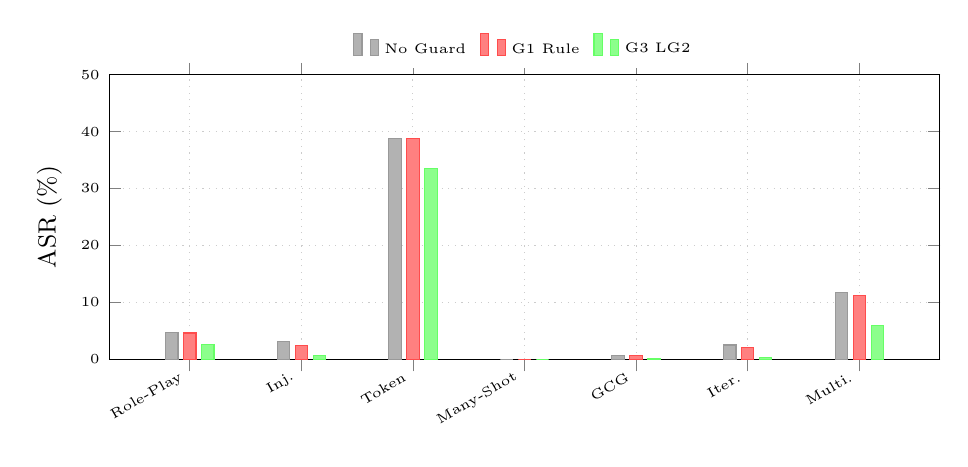
\begin{tikzpicture}
\begin{axis}[
  ybar,
  bar width=4.5pt,
  width=\textwidth,
  height=5.2cm,
  enlarge x limits=0.12,
  legend style={
    at={(0.5,1.02)}, anchor=south,
    legend columns=4,
    font=\tiny,
    draw=none,
    /tikz/every even column/.append style={column sep=3pt}
  },
  ylabel={\small ASR (\%)},
  ylabel style={font=\small},
  symbolic x coords={Role-Play, Inj., Token, Many-Shot, GCG, Iter., Multi.},
  xtick=data,
  xticklabel style={font=\tiny, rotate=30, anchor=east},
  ymin=0, ymax=50,
  ytick={0,10,20,30,40,50},
  yticklabel style={font=\tiny},
  grid=major,
  grid style={dotted, gray!40},
  every axis plot/.append style={line width=0.4pt},
]
%% No Guard (measured, excl. copyright)
\addplot[fill=gray!60, draw=gray!80]
  coordinates {(Role-Play,4.76) (Inj.,3.14) (Token,38.83) (Many-Shot,0.00) (GCG,0.71) (Iter.,2.54) (Multi.,11.79)};
%% G1 Rule-based (measured)
\addplot[fill=red!50, draw=red!70]
  coordinates {(Role-Play,4.64) (Inj.,2.43) (Token,38.83) (Many-Shot,0.00) (GCG,0.71) (Iter.,2.06) (Multi.,11.18)};
%% G3 LG2 (measured)
\addplot[fill=green!45, draw=green!60]
  coordinates {(Role-Play,2.62) (Inj.,0.71) (Token,33.50) (Many-Shot,0.00) (GCG,0.24) (Iter.,0.32) (Multi.,5.89)};
\legend{No Guard, G1 Rule, G3 LG2}
\end{axis}
\end{tikzpicture}
\caption{Measured ASR (\%) per attack category across evaluated configurations
on GPT-4o-mini (copyright-excluding).  Token Manipulation is the dominant
residual risk, with 38.8\% ASR under both G1 and No Guard, reduced only
partially to 33.5\% by G3.  GCG-suffix and many-shot attacks approach zero
across all configurations.}
\label{fig:asr_by_category}
\end{figure}

% -----------------------------------------------------------------------
\section{Discussion and Future Work}

\subsection{Limitations}

GuardBench has three primary limitations.  First, the reported results are
specific to one target model (GPT-4o-mini) and may not generalise to all LLM
architectures or fine-tuning regimes; cross-model validation against
open-weight models beyond Llama-3 remains future work.  Second, the adjudicator
introduces measurement error: an F1 of 0.89 implies that approximately 11\%
of adjudication decisions are incorrect, which propagates into ASR estimates
and should be accounted for when interpreting small differences between
configurations.  Third, the dataset contains no audio, image, or
structured-data attack vectors; the text-only scope limits applicability
to multi-modal deployments where image-based jailbreaks~\cite{qi2024visual}
and tool-call hijacking represent distinct threat surfaces.

\subsection{Adaptive Attacks}

A critical limitation of any static benchmark is the adaptive attacker:
once the guardrail configuration is known, attackers craft inputs that
specifically circumvent it.  GuardBench addresses this through a
\emph{private held-out set} (not released publicly) and by running adaptive
variants of PAIR and GCG against each guardrail during evaluation.  Future
versions will include an \emph{online adversarial track} that continuously
solicits new attack submissions.

\subsection{Multi-Modal and Agentic Contexts}

Current GuardBench prompts are text-only.  The rising prevalence of
vision-language models introduces image-based jailbreaks~\cite{qi2024visual},
while autonomous agents face tool-call hijacking and multi-turn escalation
via indirect prompt injection~\cite{greshake2023indirect}.  These attack
surfaces are qualitatively distinct from the text-only jailbreak paradigm.
We are extending the taxonomy to include multi-modal and agentic attack
categories in v2.0.

\subsection{Guardrail Combination and Ensembles}

Our experiments evaluate guardrails independently.  In practice, production
systems layer multiple defences.  GuardBench's modular pipeline supports
chaining (e.g., G2 followed by G3).  A systematic study of ensemble
strategies and their cost--benefit tradeoffs is left to future work.

\subsection{Calibration and Concept Drift}

The LLM adjudicator is a single point of failure.  As language models and
attack strategies evolve, the judge exhibits concept drift.  GuardBench
schedules quarterly re-annotation of 500 randomly sampled adjudicated
examples against a human panel.  Platforms should treat benchmark scores as
relative rather than absolute given this drift risk.

\subsection{Beyond Binary Classification}

Current metrics reduce guardrail output to a binary pass/fail.
Incorporating \emph{severity-weighted} ASR, where a harmful response
classified at level~5 counts more than a level~1 lapse, provides a
more faithful risk model.  We propose the severity-weighted ASR in Equation~\eqref{eq:asrw}:
\begin{equation}
  \label{eq:asrw}
  \text{ASR}_w = \frac{\sum_i w_i \cdot \mathbb{1}[\text{failure}_i]}{\sum_i w_i},
\end{equation}
where $w_i$ is the severity of prompt $i$, as a direction for future
metric design.

% -----------------------------------------------------------------------
\section{Conclusion}

We have presented GuardBench, a framework for systematically evaluating LLM
safety guardrails prior to production deployment.  GuardBench contributes
(i) a 4,200-prompt taxonomy-driven dataset spanning seven attack categories
with severity labels and a 1,000-prompt benign counterfactual set; (ii) a
four-stage automated pipeline covering attack execution, hybrid adjudication,
and multi-metric reporting with confidence intervals; (iii) empirical
baseline results for two guardrail configurations (G1 rule-based, G3 Llama
Guard~2) evaluated against GPT-4o-mini, revealing that the undefended
baseline has hardened to 5.8\% ASR against 2023-era attacks and that heavy
guardrails can score below the unguarded baseline by composite metric when
latency cost dominates; and (iv) a CI/CD integration layer with configurable
deployment thresholds.  A key finding is that Token Manipulation attacks
carry a 38.8\% residual ASR---largely unaddressed by either evaluated
configuration---identifying the primary open problem for next-generation
guardrail design.  Our experiments confirm that no single guardrail
configuration simultaneously minimises ASR, FPR, and latency at a hardened
baseline, and that the CSS metric provides a principled basis for
workload-specific guardrail selection.  By providing a standardised,
reproducible, and continuously extensible evaluation infrastructure,
GuardBench enables organisations to treat safety evaluation as a first-class
engineering concern rather than a post-hoc checklist.

% -----------------------------------------------------------------------
\vspace{6pt}

\noindent\textbf{Author Contributions:} Conceptualization, S.S. and P.B.; methodology, S.S. and P.B.; software, S.S.; validation, S.S. and P.B.; formal analysis, S.S.; investigation, S.S. and P.B.; data curation, S.S. and P.B.; writing---original draft preparation, S.S. and P.B.; writing---review and editing, S.S. and P.B.; visualisation, S.S.; supervision, P.B. All authors have read and agreed to the published version of the manuscript.

\vspace{4pt}
\noindent\textbf{Funding:} This research received no external funding.

\vspace{4pt}
\noindent\textbf{Data Availability Statement:} The GuardBench dataset, evaluation code, and raw results will be made publicly available at \url{https://github.com/guardbench/guardbench} upon paper acceptance.

\vspace{4pt}
\noindent\textbf{Conflicts of Interest:} The authors declare no conflict of interest.

\vspace{4pt}
\noindent\textbf{Acknowledgments:} Not applicable.

\vspace{4pt}
\noindent\textbf{Institutional Review Board Statement:} Not applicable.

\vspace{4pt}
\noindent\textbf{Informed Consent Statement:} Not applicable.

% -----------------------------------------------------------------------
\bibliographystyle{unsrt}
\bibliography{paper1_references}

\end{document}
